\documentclass[11pt]{article}
\usepackage[margin=1in]{geometry}
\usepackage{amsmath,amssymb,amsthm}
\usepackage{hyperref}
\usepackage{xcolor}
\usepackage{tikz}
\usetikzlibrary{positioning,shapes.geometric}

\newtheorem{theorem}{Theorem}
\newtheorem{definition}{Definition}
\newtheorem{example}{Example}
\newtheorem{remark}{Remark}

\newcommand{\Z}{\mathbb{Z}}
\newcommand{\R}{\mathbb{R}}
\DeclareMathOperator{\coker}{coker}
\DeclareMathOperator{\im}{im}

\title{Understanding the Pentagon Game:\\Chip-Firing on the $R_{10}$ Matroid}
\author{Implementation Guide}
\date{\today}

\begin{document}

\maketitle

\begin{abstract}
This document explains the mathematical foundations of our Pentagon Game implementation, connecting the playable game to the deep mathematics of chip-firing on the $R_{10}$ matroid. We explain \emph{why} this particular game structure matters, how it relates to Alex McDonough's research, and what the code is actually computing.
\end{abstract}

\section{The Big Picture: Why Study Chip-Firing?}

\subsection{What is Chip-Firing?}

Chip-firing is a discrete dynamical system that appears in multiple areas of mathematics:

\begin{itemize}
    \item \textbf{Combinatorics}: Counting spanning trees and graph structures
    \item \textbf{Algebra}: Understanding finite abelian groups
    \item \textbf{Physics}: Modeling self-organized criticality (sandpiles, earthquakes)
    \item \textbf{Algebraic Geometry}: Discrete analogs of divisors on Riemann surfaces
\end{itemize}

\textbf{Core Idea:} Simple local rules (firing chips between neighbors) lead to complex global behavior (group structure, equivalence classes).

\subsection{The Sandpile Group}

For a connected graph $G$ with $n$ vertices, the \textbf{sandpile group} $S(G)$ is a finite abelian group with a remarkable property:

\begin{theorem}[Matrix-Tree Theorem Connection]
The order of the sandpile group equals the number of spanning trees:
\[
|S(G)| = \text{number of spanning trees of } G
\]
\end{theorem}

The sandpile group captures the \emph{algebraic essence} of the graph's structure.

\section{Why $R_{10}$? Seymour's Decomposition}

\subsection{Matroids: Generalized Independence}

A \textbf{matroid} is an abstraction of the concept of ``linear independence.'' While graphs give us one type of matroid (graphic matroids), there are others.

\begin{definition}[Regular Matroid]
A \textbf{regular matroid} is one that can be represented by a totally unimodular matrix over $\R$, where all minors are in $\{-1, 0, 1\}$.
\end{definition}

\subsection{Seymour's Fundamental Theorem}

\begin{theorem}[Seymour 1980]
Every regular matroid can be built from three basic building blocks using sums:
\begin{enumerate}
    \item Graphic matroids (from graphs)
    \item Cographic matroids (from dual graphs)
    \item \textbf{$R_{10}$} (a specific 10-element, rank-5 matroid)
\end{enumerate}
\end{theorem}

\textbf{Analogy:} Just as every integer is built from prime numbers, every regular matroid is built from these three types. $R_{10}$ is like a ``prime matroid.''

\textbf{Why this matters:} Understanding chip-firing on $R_{10}$ helps us understand chip-firing on \emph{all} regular matroids!

\section{The Pentagon Structure: From 10D to 5D}

\subsection{Standard Representation}

The matroid $R_{10}$ is standardly represented as a $5 \times 10$ matrix:
\[
\mathcal{A} = \begin{bmatrix}
    1 & 0 & 0 & 0 & 0 &   -1 & 1 & 0 & 0 & 1\\
    0 & 1 & 0 & 0 & 0 &   1 & -1 & 1 & 0 & 0\\
    0 & 0 & 1 & 0 & 0 &   0 & 1 & -1 & 1 & 0\\
    0 & 0 & 0 & 1 & 0 &   0 & 0 & 1 & -1 & 1\\
    0 & 0 & 0 & 0 & 1 &   1 & 0 & 0 & 1 & -1
\end{bmatrix}
\]

Chip configurations live in $\Z^{10}$ - that's 10 dimensions!

\subsection{The Gaussian Integer Trick}

Alex McDonough's key insight: The matrix $\mathcal{D}$ (the second half of $\mathcal{A}$) is \emph{symmetric}, which allows a clever representation using \textbf{Gaussian integers} $\Z[i] = \{a + bi : a,b \in \Z\}$.

Define the bijection:
\[
\varphi: \Z^{10} \to \Z[i]^5, \quad (v_0,\ldots,v_9) \mapsto (v_0 + v_5i,~ v_1 + v_6i,~ v_2 + v_7i,~ v_3 + v_8i,~ v_4 + v_9i)
\]

This groups each pair of coordinates into a single complex number!

\subsection{The Pentagon Emerges}

In the $\Z[i]^5$ representation, the firing moves act on a \textbf{pentagon graph}:

\begin{center}
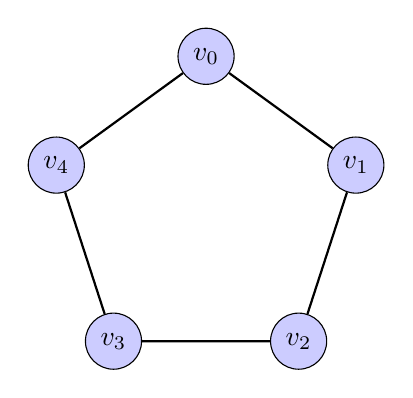
\begin{tikzpicture}[scale=2]
    \node[circle,draw,fill=blue!20] (v0) at (90:1) {$v_0$};
    \node[circle,draw,fill=blue!20] (v1) at (90-72:1) {$v_1$};
    \node[circle,draw,fill=blue!20] (v2) at (90-144:1) {$v_2$};
    \node[circle,draw,fill=blue!20] (v3) at (90-216:1) {$v_3$};
    \node[circle,draw,fill=blue!20] (v4) at (90-288:1) {$v_4$};

    \draw[thick] (v0) -- (v1) -- (v2) -- (v3) -- (v4) -- (v0);
\end{tikzpicture}
\end{center}

Each vertex is connected to exactly 2 neighbors (cycle graph $C_5$).

\section{The Four Moves: A, B, C, D}

\subsection{Move Definitions}

The complex number representation gives us four fundamental firing moves:

\begin{definition}[The Four Moves]
\begin{enumerate}[(A)]
    \item \textbf{Move A:} Add $1+i$ to the selected vertex, add $-i$ to each of its 2 neighbors
    \item \textbf{Move B:} Add $-1+i$ to the selected vertex, add $1$ to each of its 2 neighbors
    \item \textbf{Move C:} Add $-1-i$ to the selected vertex, add $i$ to each of its 2 neighbors
    \item \textbf{Move D:} Add $1-i$ to the selected vertex, add $-1$ to each of its 2 neighbors
\end{enumerate}
\end{definition}

\subsection{Relationship Between Moves}

Notice the beautiful pattern:
\begin{align*}
\text{Move C} &= -(\text{Move A}) \\
\text{Move D} &= -(\text{Move B})
\end{align*}

This is why our UI only shows buttons for A and B - the negatives are accessed via right-click!

\subsection{Why These Specific Moves?}

These moves come from the matrix $\overline{\mathcal{K}} = I_5 - \mathcal{D}i$:
\[
\overline{\mathcal{K}} = \begin{bmatrix}
    1 + i & -i & 0 & 0 & -i \\
    -i & 1 + i & -i & 0 & 0 \\
    0 & -i & 1 + i & -i & 0 \\
    0 & 0 & -i & 1 + i & -i \\
    -i & 0 & 0 & -i & 1 + i
\end{bmatrix}
\]

Firing at vertex $v_j$ corresponds to subtracting the $j$-th row of $\overline{\mathcal{K}}$ from the configuration vector.

\section{The 162 Equivalence Classes}

\subsection{The Sandpile Group Structure}

\begin{theorem}[Structure of $S(R_{10})$]
The sandpile group of $R_{10}$ is isomorphic to:
\[
S(R_{10}) \cong (\Z/3\Z)^3 \oplus (\Z/6\Z)
\]
\end{theorem}

\textbf{Counting:} $|S(R_{10})| = 3 \times 3 \times 3 \times 6 = 162$

\subsection{What Are These Equivalence Classes?}

Two chip configurations $c$ and $c'$ are \textbf{firing equivalent} (written $c \sim c'$) if one can be reached from the other by a sequence of A, B, C, D moves.

The sandpile group is the quotient:
\[
S(R_{10}) = \frac{\Z[i]^5}{\im(\overline{\mathcal{K}})}
\]

\textbf{Physical Interpretation:} The 162 equivalence classes represent the 162 ``fundamentally different'' chip configurations. All others are just these 162 repeated.

\subsection{The Unique Element of Order 2}

The group $S(R_{10})$ has exactly \textbf{one element of order 2}, denoted $H$:
\[
H + H = 0 \text{ (in the group)}
\]

In Alex's paper, he identifies which configurations satisfy $c \sim H$.

\section{Our Implementation: Code Meets Mathematics}

\subsection{Data Structures}

\textbf{Complex Number:}
\begin{verbatim}
interface ComplexNumber {
  real: number;
  imag: number;
}
\end{verbatim}

\textbf{Game State:}
\begin{verbatim}
interface GameState {
  vertices: ComplexNumber[5];     // Pentagon configuration
  currentMoveType: 'A'|'B'|'C'|'D';
  goalVertices: ComplexNumber[5]; // Always [0,0,0,0,0]
  isWon: boolean;
}
\end{verbatim}

\subsection{Move Implementation}

The move definitions match the paper exactly (after bug fixes!):

\begin{verbatim}
const moves = {
  'A': { vertex: {real: 1, imag: 1}, adjacent: {real: 0, imag: -1} },
  'B': { vertex: {real: -1, imag: 1}, adjacent: {real: 1, imag: 0} },
  'C': { vertex: {real: -1, imag: -1}, adjacent: {real: 0, imag: 1} },
  'D': { vertex: {real: 1, imag: -1}, adjacent: {real: -1, imag: 0} },
};

const adjacency = {
  0: [1, 4],  // v0 connects to v1 and v4
  1: [0, 2],  // v1 connects to v0 and v2
  2: [1, 3],  // etc.
  3: [2, 4],
  4: [3, 0],
};
\end{verbatim}

\textbf{Critical Bug Fixed:} Initially, we had the real and imaginary parts swapped for adjacent vertices. The paper specifies move A adds $-i$ (imaginary) to neighbors, not $-1$ (real)!

\subsection{The Matrix Solver}

We use $\overline{\mathcal{K}}^{-1}$ to find optimal moves:

\[
\overline{\mathcal{K}}^{-1} = \frac{1}{6}\begin{bmatrix}
    3 - i & 1 + i & -1 + i & -1 + i & 1 + i \\
    1 + i & 3 - i & 1 + i & -1 + i & -1 + i \\
    -1 + i & 1 + i & 3 - i & 1 + i & -1 + i \\
    -1 + i & -1 + i & 1 + i & 3 - i & 1 + i \\
    1 + i & -1 + i & -1 + i & 1 + i & 3 - i
\end{bmatrix}
\]

\textbf{Hint Algorithm:}
\begin{enumerate}
    \item Compute difference vector: $d = 0 - c$ (goal minus current)
    \item Apply inverse: $s = \overline{\mathcal{K}}^{-1} \cdot d$
    \item Test all 20 moves (4 types $\times$ 5 vertices)
    \item Return move that minimizes distance to zero
\end{enumerate}

\textbf{Note:} This is a \emph{greedy} approach (one-step lookahead), not guaranteed optimal for all puzzles.

\section{What's Different from Classic Chip-Firing?}

\subsection{Classic Chip-Firing (Graphs)}

\textbf{Rules:}
\begin{itemize}
    \item Vertex fires when $\text{chips}(v) \geq \deg(v)$
    \item Firing is automatic/required
    \item Process continues until stable
\end{itemize}

\textbf{Goal:} Understand which configurations stabilize

\subsection{Our Game ($R_{10}$ Variant)}

\textbf{Rules:}
\begin{itemize}
    \item Player chooses which move (A/B/C/D) and where
    \item Moves have fixed effects (not threshold-based)
    \item Complex number arithmetic
\end{itemize}

\textbf{Goal:} Reach the zero configuration $[0, 0, 0, 0, 0]$

\subsection{Key Insight}

Our game is not about \emph{automatic stabilization} - it's about exploring the \textbf{equivalence classes} of the sandpile group!

Each puzzle starts in one of the 162 orbits. The question is: which moves bring you to the zero configuration (if possible)?

\section{Open Questions \& Future Work}

\subsection{What We Know}

\begin{itemize}
    \item The move definitions are mathematically correct $\checkmark$
    \item The matrix solver uses the correct $\overline{\mathcal{K}}^{-1}$ $\checkmark$
    \item The pentagon adjacency is correct $\checkmark$
    \item Puzzles are generated using random coefficient combinations $\checkmark$
\end{itemize}

\subsection{What We Don't Show (Yet)}

\begin{enumerate}
    \item \textbf{Orbit Number:} Which of the 162 equivalence classes is the current configuration in?
    \item \textbf{Representatives:} Display all 162 representative configurations
    \item \textbf{Solvability:} Is the current puzzle actually solvable, or are we in the wrong orbit?
    \item \textbf{Optimal Path:} The greedy solver may not find the shortest solution
\end{enumerate}

\subsection{Computing the Orbit}

To determine which equivalence class a configuration $c$ belongs to, we need to compute:
\[
c \mod \im(\overline{\mathcal{K}})
\]

This requires:
\begin{itemize}
    \item Computing a Hermite normal form of $\overline{\mathcal{K}}$
    \item Finding a set of 162 canonical representatives
    \item Reducing $c$ to one of these representatives
\end{itemize}

\textbf{Challenge:} This is computationally complex and not yet implemented!

\section{Conclusion: Why This Game Matters}

\subsection{For Mathematics}

This game provides a \textbf{concrete, interactive demonstration} of:
\begin{itemize}
    \item Chip-firing on a non-graphic matroid
    \item The 162-orbit structure of $S(R_{10})$
    \item The Gaussian integer representation trick
    \item Matrix-based solver approaches
\end{itemize}

\subsection{For Learning}

The game makes abstract algebra \textbf{tangible}:
\begin{itemize}
    \item See group equivalence classes in action
    \item Understand why certain moves ``cancel out''
    \item Experience the difference between solvable and unsolvable configurations
    \item Visualize complex number arithmetic geometrically
\end{itemize}

\subsection{The Big Takeaway}

\begin{center}
\fbox{\parbox{0.9\textwidth}{
\textbf{Key Insight:} What looks like a simple number puzzle is actually a playable demonstration of deep mathematics connecting matroid theory, algebraic topology, and group theory.

The pentagon isn't random - it's the natural structure that emerges when you represent $R_{10}$ using Gaussian integers!
}}
\end{center}

\section*{Acknowledgments}

This implementation is based on the mathematical framework developed by Alex McDonough in his paper ``Chip-Firing and the Sandpile Group of the $R_{10}$ Matroid.'' All mathematical credit goes to Alex and the broader chip-firing research community.

\end{document}
